\chapter{Protein Overview}
\label{sec:protein-overview}

A brief introduction to proteins is given in Sect.\ref{sec:proteins-evolution}.

\section{Evolution of Proteins}
\label{sec:evolution-proteins}
\label{sec:proteins-evolution}

Proteins (Sect.\ref{sec:protein-overview}) are special biomolecules
(Sect.\ref{sec:biomolecule}), and play crucial structural and functional roles
in organism's body: structures, muscle contraction, nerve impulses, hormone
action, chemical signaling, and regulation of metabolism.  Proteins are
synthesized from 20 different monomers called amino acids, ranging in number
from about 50 to 2000 amino acids per protein. Proteins are synthesized at a
cellular structure known as ribosomes.

The instruction of how to build a protein is encoded by genes which are segments
in the DNA (Sect.\ref{sec:dna}). DNA contains life-encoding information, and
exist in the form of double-strands structure, twisted to reduce the occupied
space in the form of chromosome (Sect.\ref{sec:chromosome}).

Each new generation of cells must have a complete set of genes inherited from
the parent cells so that one copy can be given to each of the two daughter cells
(from cell division). Also the cell has tricks for producing different versions
of proteins form a single gene ({\bf differential splicing technique} -
Sect.\ref{sec:splice-variant}). 

\begin{mdframed}
Each cell contains the full gene set. However, depending on the cell types,
certain genes are expressed only. A human being has an estimated 30,000 genes in
each cell.

\end{mdframed}


Another point is that with a large number of genes, the duplication
(reproduction) of this vast mass of information cannot occur without
errors which are known as gene mutations. The gene changes causes a
new protein is created. This process is called
{\bf evolution of protein}.

The evolution of protein requires the development of new genes. The
problem is that how you can change an essential gene to a new one
without eliminating the function of the original gene? It can be
explained by another type of accident in the replication of genes,
namely {\bf gene duplication} in which a given gene is duplicated
twice. From this we have the evidence that a set of related genes
exists which obviously have evolved from a common ancestor.



\section{Protein length and size}
\label{sec:protein-length}
\label{sec:protein-size}

The protein size can be measured geometrically in terms of how much space they
take up and in terms of their sequence size as determined by the number of amino
acids that are strung together to make the protein.

NOTE: average amino acid has a molecular mass of 100 Da, we can easily
interconvert between mass and sequence length.

\begin{enumerate}
  
  \item Rubisco protein (monomeric mass 55 kDa):  one of the most abundant
  proteins on Earth, is responsible for extracting about a hundred Gigatons of
  carbon from the atmosphere each year

  For example the 55 kDa Rubisco monomer, has roughly 500 amino acids making up
  its polypeptide chain. By fixating CO2 one at a time, with each CO2 with a
  mass of 0.044 kDa (just another way of writing 44 Da that clarifies the 1000:1
  ratio in mass).
  
  
  \item ATP synthase (molecular mass 500-600 kDa): decorates our mitochondrial
  membranes and is responsible for synthesizing the ATP molecules (with mass
  507 Da - Sect.\ref{sec:ATP-molecule})
  
  \item 
\end{enumerate}
Unlike Rubisco protein which can function as a monomer, 
in half the number of proteins, it turns out that proteins function when several
identical copies are symmetrically bound to each other, e.g. homo-olimers or
hetero-olimers. Homo-oligomers are about twice as common as hetero-oligomers.
The most common states are the dimer and tetramer (and the non
oligomeric monomers). 

Median length of proteins
\begin{verbatim}
H. sapiens				375 a.a
D. melanogaster			373 a.a.
C. elegans				344 a.a.
S. cerevisiae 			379 a.a.
A. thaliana				356 a.a.
eukaryotes				361 a.a.
bacteria				267
archaea 				247 a.a.
\end{verbatim}

\subsection{volume and diameter}

The spatial extent of soluble proteins and their sequence size often exhibit an
approximate scaling property 
\begin{enumerate}
  \item  volume scales linearly with sequence size  	
  
  Thus the radii or diameters tend to scale as the sequence size to the 1/3
  power.
 
 Example: Rubisco protein is  3-6 nm in diameter.
  
  \item 
\end{enumerate}

\url{http://book.bionumbers.org/how-big-is-the-average-protein/}

\section{Reelin}
\label{sec:reelin}


Reelin is a large secreted extracellular matrix glycoprotein that helps regulate
the neuronal migration and positioning of cells in the developing brain by
controlling cell-cell interactions (Sect.\ref{sec:Cajal-Reizius-cell}).

Reelin continues to work in the adult brain. It modulates synaptic plasticity by
enhancing the induction and maintenance of long-term potentiation, stimulate
dendrite and dendritic spines development, \ldots
\url{https://en.wikipedia.org/wiki/Reelin}

\section{Protein regulation: covalent modification}
\label{sec:protein-regulation}
\label{sec:covalent-modification}

Covalent modification has been identified with control in carbohydrate
metabolism, fat metabolism, sensory systems, muscular contraction, protein
synthesis, nitrogen metabolism, and malignant transformation.

Proteins that have been found to be controlled by covalent modification
(leading to 2 forms: phosphorylated and dephosphorylated), i.e.
protein can exist in the unmodified form W and the modified
form W*.
\begin{enumerate}
  \item glycogen phosphorylase : Cori and Green (1) and Krebs and
Fischer (2)
  
  \item IP3 - Sect.\ref{sec:IP3-degradation}
\end{enumerate}

\subsection{sensitivies}
\label{sec:sensitivies}

In phenomena such as sensing, and in the regulation of metabolism, it is
important that the "turning on" of one pathway and the "turning off" of another
be sensitive to relatively small changes in effector concentration

\begin{enumerate}
  
  \item  One known mechanism for increasing the sensitivity of a system is
  through cooperative interactions. - Sect.\ref{sec:cooperativity}

  \item Another is the effect of a ligand that enters at more than one step in a
  pathway-e.g., to activate one enzyme and inhibit another, as happens in the glycogen cascade

  \item there is a property of covalent systems that, in the absence of
  allosteric cooperativity and multiple inputs, can generate sensitivity
  equivalent to cooperative enzymes with high Hill coefficients.

The response can arise from kinetics of covalent modification analogous to the
cooperativity present in allosteric enzymes with, Hill coefficients greater than
1.

\label{sec:stochastic-resonance}
This is called {\bf ultra-sensitivity}, to describe
an output response that is more sensitive to change in
stimulus than the hyperbolic (Michaelis-Menten) equation -
Sect.\ref{sec:Michaelis-Menten-modified}.
Other name is {\bf stochastic resonance}.
\url{https://en.wikipedia.org/wiki/Stochastic_resonance_(sensory_neurobiology)}
\end{enumerate}

\subsection{splice variants}
\label{sec:splice-variant}



\section{Protein components}
\label{sec:protein-components}

\subsection{-- inside CSF}
\label{sec:protein-components-CSF}

The protein concentration in CSF increases with age, and reaches up to 600 mg/L
in old age without clinical relevance (Rice \& Singer, 1965).

Lumbar CSF contains slightly higher protein amounts than suboccipital CSF, with
244 mg/L compared to 218 mg/L, respectively.


\section{Protein domains}

A protein is made of a sequence of amino acids ({\bf primary structure}),
Fig.\ref{fig:protein-structure-4-levels}.

A short segments of amino acids interact to each other and form {\bf secondary
structures}
\begin{enumerate}
  \item alpha helices
  
  \item beta pleated sheets
  
  \item 
\end{enumerate}

An overal 3D structure of all segments form the {\bf tertiary structure}.

When two or more poly-peptides that are folded in 3D shape and combine together,
we have {\bf quaternary structure}.

\begin{figure}[hbt]
  \centerline{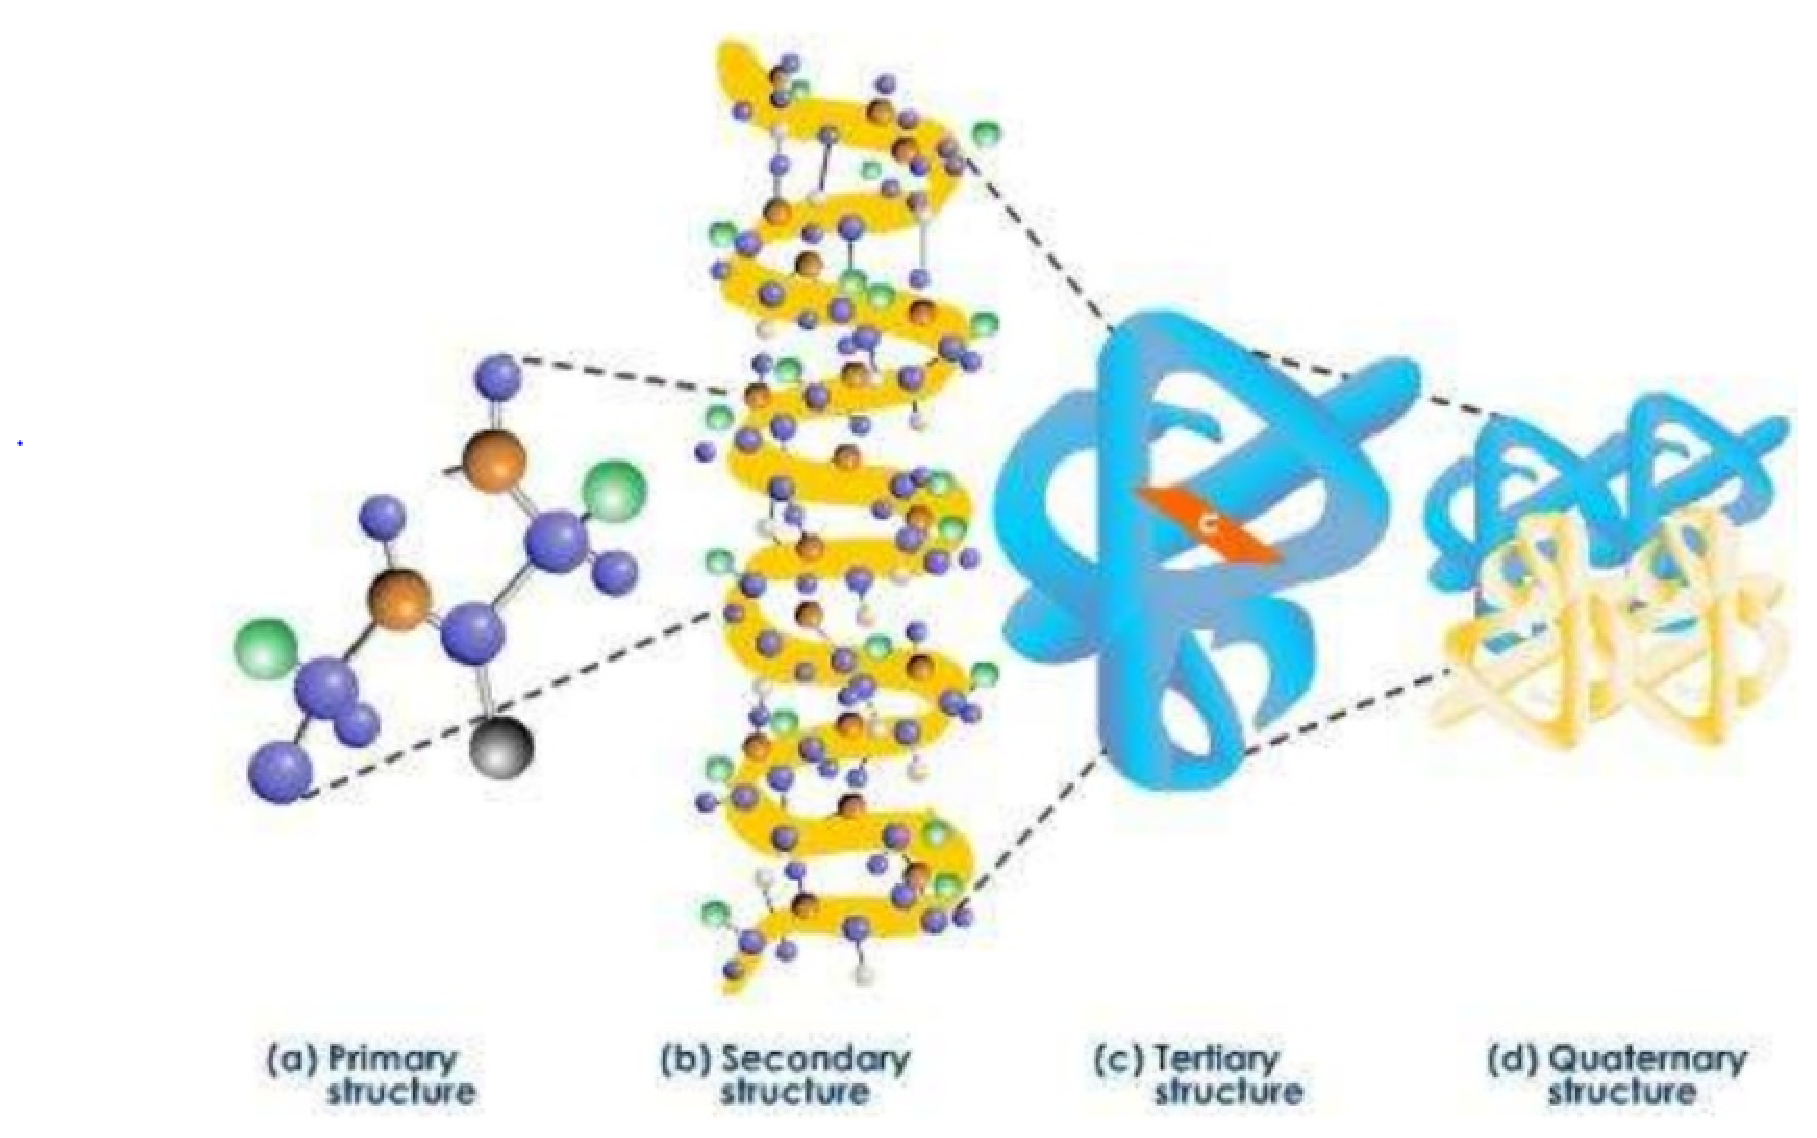
\includegraphics[height=4cm,
    angle=0]{./images/protein-structure-4-levels.eps}}
  \caption{Protein 4 levels of structures}
  \label{fig:protein-structure-4-levels}
\end{figure}


\subsection{HEAT repeat}
\label{sec:HEAT-repeat}

The term HEAT for HEAT repeat domain comes from the first 4 proteins that
were found containing this domain: ({\bf H}untingtin, elongation factor 3 ({\bf
E}F3), protein phosphatase 2A (PP2{\bf A}), and the yeast kinase {\bf T}OR1).
See Sect.\ref{sec:Htt-protein} for Huntington protein.

HEAT repeat domain consists repeats of about 47 residues that forms 2
anti-parallel $\alpha$-helix and two turns arranged about the common axis. These
repeats are linked by flexible inter-unit loops.
%, with 10-35 glutamates

FUNCTION: There are evidences suggested domains formed by HEAT-repeats are
important for the formation of protein-protein interactions.
% a rod-like helical structures which are involved in
% intracellular transport
\url{http://pawsonlab.mshri.on.ca/index.php?option=com_content&task=view&Itemid=64&id=203}


\section{Histone deacetylase: HDAC (KDAC)}
\label{sec:HDAC}
\label{sec:KDAC}
\label{sec:Histone-deacetylase}

{\bf TIPS:} Histone is a type of proteins that packs the long chain of DNA into
bead-like structures of the chromosome (Sect.\ref{sec:histone}). To transcribe a
region of DNA sequence, histone need to be removed from the DNA sequence which
is done by the enzyme called HAT {\bf histone deacetylases} (HAT) -
Sect.\ref{sec:HAT}. In particular, HAT carries out lysine acetylation on histone
(Sect.\ref{sec:histone}). In opposite, HDAC reverse lysine acetylation, i.e.
lysine deacetylation, from N-terminal of histone, allowing the histone to wrap
more tightly, i.e. preventing gene transcription.


IMPORTANT: As HDAC also target non-histone proteins, HDAC proteins are now also
called {\bf lysine deacetylases} (KDAC), to describe their function rather than
their targets which are multiple. \textcolor{red}{\it There are more than 50
non-histone proteins identified as substrate for HDAC.}

\begin{enumerate}
  \item classes of HDAC - Sect.\ref{sec:HDAC-classes}

The zinc ion located at the bottom of HDAC's conserved deep channel structure.
Many HDACs perform its lysine deactylase function in a zinc-dependent catalytic
action. These HDACs are classified into Class I, II and IV. 
  
  \item HDAC affinity to targets - Sect.\ref{sec:HDAC-affinity}
\end{enumerate}

\subsection{isoforms/classes}
\label{sec:HDAC-classes}

In mamals, there are 18 found HDAC.

The HDACs are phylgenetically classied into 4 classes of HDAC, depending upon
their sequence similarity with homologous enzymes from {\it Saccharomyces
cerevisiae}: each with different members
\begin{enumerate}
  \item Class I HDAC: 4 members - HDAC1-3; and HDAC8
  
  Enzymes of Class I and Class II HDAC are closely related to yeast {\bf scRdp3}
  and {\bf scHda1}, respectively. 
  
  \textcolor{red}{Class I HDACs} are involved in cell proliferation
  and survival; and are expressed ubiquitously in different body tissues. 
    
  \item Class IIA HDAC: 4 members - HDAC4, HDAC5, HDAC7, and HDAC9
  
  Members in Class IIA can shuttle between cytoplasm and nucleus; with weaker
  deacetylase activity.
  
  \item Class IIB HDAC: 2 members - HDAC6 (Sect.\ref{sec:HDAC6}) and HDAC10
  (Sect.\ref{sec:HDAC10})
  
  Classes IIB is mostly found in cytosol; with a preference targeting to
  non-histone proteins.
  The members has two catalytic domains.
  
  
  \textcolor{red}{Class II HDAC seems to have tissue-specific role}; depending
  the non-histone protein target.
   
  \item Class III HDAC (known as {\bf sirtuins}): are homologous to yeast {\bf
  scSir2}. 
  
  Enzymes in Class III HDAC requires a specific cofactor (NAD+ -
  Sect.\ref{sec:NAD+}) for activity, with different structural features.
  
  \item Class IV HDAC: only 1 member: HDAC11

HDAC11 was found closely related to class I; yet not enought identity to be
placed in it; so it is put into a new class.

\end{enumerate}

\subsection{structure}
\label{sec:HDAC-structure}

The first HDAC-like protein structure solved by X-ray was the bacterial HDAC
homologue HDLP from {\it Aquifex aelicus} in 1999.

Structural analysis revealed a conserved 11 $\AA$ deep channel among all HDAC
structures; with zinc ion located at the bottom. Class I, II, and IV HDACs
depend on zinc to perform its function,  i.e. zinc-dependent HDACs.

4 members of Class I HDAC are ubiquitous, and relatively small enzymes (about
500 amino acids) essentially located in nucleus of the cells.

6 members of Class II HDAC are larger (about 1000 amino acids) and are further
classified into Class IIA and IIB. 
\begin{itemize}
  \item N-terminal of class IIA is the one responsible for nuclear-cytoplasmic
  shuttling through phosphorylation-dependent binding to 14-3-3 proteins.
  
  This interaciton regulates the activity of transcription factor such as 
  myocyte enhancer factor-2 (MEF2) - play repressor role in a variety of
  biological functions.
  
  \item 
\end{itemize}



\subsection{affinity/specificity}
\label{sec:HDAC-affinity}

In general, HDACs have a relatively low substrate specificity, i.e. a single
enzyme can deacetylate multiple sites of histones.

NOTE: HDACs are often found to be together in multiple distinct complexes.
This makes it difficult to determine which activity (specific HDAC and/or
complex) is responsible for a specific effect.
\begin{enumerate}
  \item HDAC1 is found with HDAC2 within NuRD, Sin3a and Co-REST complexes
  
  HDAC1, HDAC2, and HDAC3 are found in complexes with specific transcriptional
  corepressors, blocking the expression of tumor suppressor genes.
  
\end{enumerate}


HDAC's role
\begin{enumerate}
  \item affect DNA reading, i.e. enhance

  \item HDAC4: affect the aggregation (i.e. sticky glob formation) of mHtt
  protein

NOTE: Get rid of HDAC4   delay the forming of sticky globs of mHtt.
HDAC4 also contains glutamine-rich region.

  \item class IIA HDAc has another zinc ion coordinated to a
Cys-Cys-His-Cys motif close to the cavity that may participate in substrate
recognition or in protein interactions.
  
  \item HDAC2: 

So, along with the NFAT nuclear import, we observe the
export of HDAC2.
  
\end{enumerate}

\subsection{HDAC10}
\label{sec:HDAC10}

HDAC10 has 2 catalytic domains; one of that is catalytically inactive domains
whose biological function is still unknown.

\subsection{HDAC4}
\label{sec:HDAC4}

HDAC4 remains sequestered in the cytoplasm until it is called upon to shuttle
into the nucleus to take part in regulating transcription.

The potential theurapeutic roles of HDAC4 have been suggested for
\begin{enumerate}
  \item HD - Sect.\ref{sec:HD-theory-HDAC-inhibitor}
\end{enumerate}



\subsection{HDAC6}
\label{sec:HDAC6}

HDAC6 is Class IIB HDAC (Sect.\ref{sec:HDAC}), with 1215 amino acids, and is
found mainly in heart, liver, kidney, placenta; with small prevelance in brain,
Fig.\ref{fig:HDAC_ClassIIB-subcellular-rat-brain}.
However, the role of HDAC in neurodegeneration has been partially elucidated so
far, particularly of beneficial in animal models of neurodegenerative diseases
(Simoes-Pires et al., 2013).
HDAC6 plays a central role in protein aggregate elimination, in neuronal
oxidative stress and in the mitochondrial transport.

\begin{figure}[hbt]
  \centerline{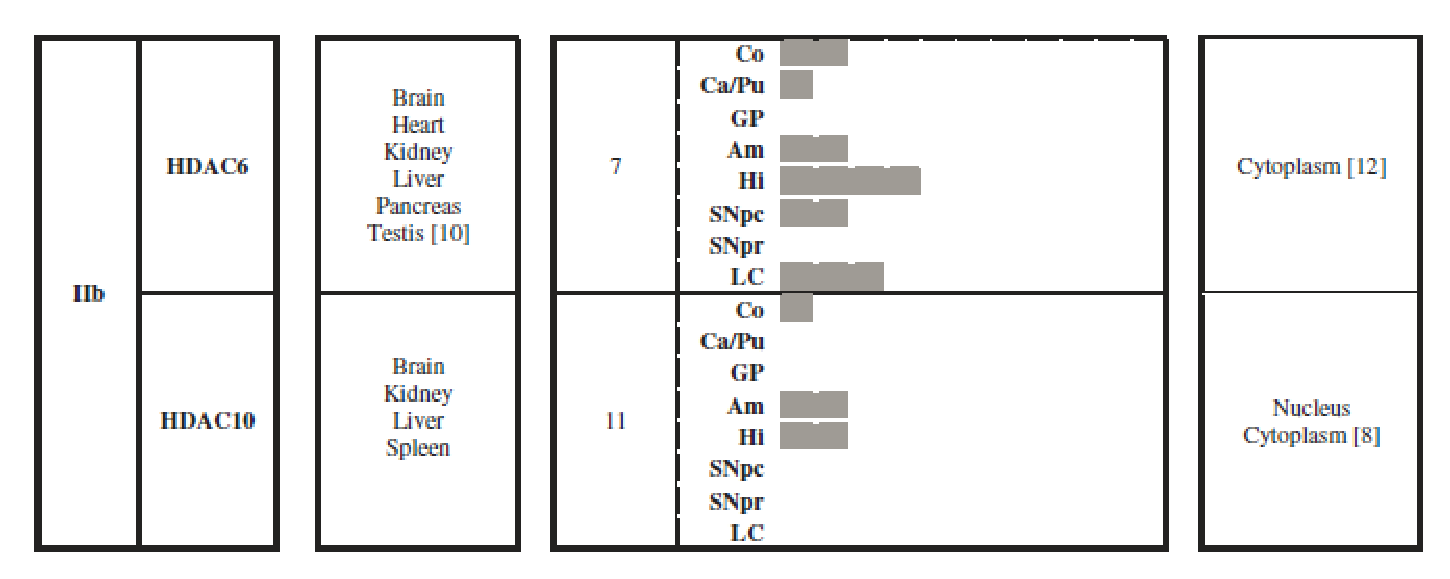
\includegraphics[height=5cm,
    angle=0]{./images/HDAC_ClassIIB-subcellular-rat-brain.eps}}
\caption{HDAC6 and HDAC10 distribution in rat brain in the scale of 10:
Co (Cortex); Ca/Pu (striatum: Caudate/Putamen); Am (Amygdala); Hi
(Hippocampus); SNpc (Sect.\ref{sec:SNpc}); LC (Locus coeruleus)}
\label{fig:HDAC_ClassIIB-subcellular-rat-brain}
\end{figure}


HDAC6 has 2 independent catalytic domains with zinc-finger ubiquitin-binding
domain at C-terminal.
\begin{itemize}
  \item a zone characterized by Ser-Glu containing tetradeca-peptide repeating
  domain (SE14): responsible for HDAC6 intracellular retention and {\it tau}
  interaction - Sect.\ref{sec:tau-protein}.
  
  \item two leucine-rich nuclear export sequence (NES1, NES2):
  control nucleus-cytoplasmic shuttling process.
  
  \item what make HDAC6 different from others is the presence of {\bf zinc
  finger domain at C-terminal}.
  
This structure  alone and in complex with ubiquitin, is formed by a compact
structure of 5 antiparallel $\beta$-strands, 2 $\alpha$-helices, and 3 zinc ions
with a distinct aromatic pocket. It is similar to other human zinc finger
domains recognizing ubiquitin (Sect.\ref{sec:ubiquitin}).

\end{itemize}

\textcolor{red}{The strategy to be adopted in promising therapeutics targeting
HDAC6 is still controversial.}

\begin{itemize}

  \item 
  HDAC/HAT enzymatic balance has been suggested to be important in neuronal
  homeostasis, such as neurophysiological functions, memory processes, and
  learning.
  
  The deregulation of this balance may affect proper gene expression of
  proteins involved in apoptosis and neuroprotection.
    
  \item    Specific inhibitors exert neuroprotection by increasing the
  acetylation levels of $\alpha$-tubulin with subsequent {\it improvement of the
  axonal transport} - Sect.\ref{sec:axonal-transport}, which is usually impaired
  in neurodegenerative disorders.
  
HDAC6 has 2 catalytic domains; and  take part in the microtubule network by
acting as a specific $\alpha$-tubulin deacetylase.
  
   \item bind to ubiquitin - Sect.\ref{sec:ubiquitin} - modulating cell
   protective response to cytotoxic accumulation of misfolded and aggregated
   proteins.
   
   
     
\end{itemize}

\subsection{HDAC6 inhibitor: tubacin}
\label{sec:HDAC6-inhibitor-tubacin}

One of the most studied HDAC6 specific inhibitor is tubacin.
\begin{enumerate}
  \item IC50 = 
\end{enumerate}

\subsection{HDAC6 inhibitor: ricolinostat}
\label{sec:HDAC6-inhibitor-ricolinostat}

The selective histone deacetylase 6 (HDAC6) inhibitor, ricolinostat, for the
treatment of multiple myeloma. Clinical results to date suggest that
ricolinostat is likely to operate synergistically with other agents.

\section{EGF (epidermal growth factor)}
\label{sec:EGF}

Epidermal growth factor (EGF) is  is a growth factor that stimulates cell
growth, proliferation, and differentiation by binding to its receptor EGFR
(Sect.\ref{sec:EGFR}).

Human EGF is a 6-kDa protein with 53 amino acid residues and three
intramolecular disulfide bonds.

EGF was first found in submaxillary glands of mice and in human urine; and then
found in many human tissues: e.g. submandibular gland, parotid gland.

\subsection{EGFR}
\label{sec:EGFR}



\section{Neurotrophin}
\label{sec:neurotrophin}

Neurotrophin refers to molecules with trophic (survival- and growth-promoting)
effects on neurons. The gene family encodes functionally and structurally
related proteins:

\begin{enumerate}
  \item NGF - Sect.\ref{sec:NGF}

NGF was the first member. The second-member of this neurotrophic family is BDNF
(Sect.\ref{sec:BDNF}). 
  
  \item BDNF - Sect.\ref{sec:BDNF}
  
  \item NT-3 (neurotrophin-3) - Sect.\ref{sec:NT-3}: or NGF-2 or
  hippocampus-derived neurotrphic factor (HDNF)

Newer members: NT-3, NT-4/5 have also been found; each
has a distinct profile of trophic effects on subpopulations of neurons in the
peripheral and central nervous systems.
  
  \item NT-4/5 - Sect.\ref{sec:NT-4/5}
\end{enumerate}
Neurotrophin effects are mediated by interaction with their heterogeneous
receptors (referred to as NGFRs - Sect.\ref{sec:NGFR}) present on specific
neuronal cell populations.

Neurotrophins also share a distinctive three-dimensional structure containing
two pairs of antiparallel $\beta$-strands and cysteine residues in a cystine
knot motif.

NOTE: Preneurotrphin have altered binding characteristics and distinct biologic
activity in comparison with mature neurotrophins.

Depending on the member, it activates a particular member of two different
receptor classes
\begin{enumerate}
  \item Trk - Sect.\ref{sec:Trk}, e.g. TrkB receptor - Sect.\ref{sec:Trk-B}
  
  \item p75 receptor - Sect.\ref{sec:p75-receptor}
\end{enumerate}

\subsection{NGF: Neuron growth factor}
\label{sec:NGF}

Levi-Montalcini and  Stanley Cohen shared the Nobel prize for finding a
compound, expressed in peripheral cells, that attracted spinal neurons and
induced neurite formation discovered in the early 1950s.
The compound is called NGF as its trophic (survival- and growth-promoting)
effects on sensory and sympathetic neurons (Levi-Montalcini and Hamburger,
1951). 

The substance - NGF - was then isolated from tumors, snake venom, and
mouse salivary glands. NGF is the first identified growth factor.
The structure of NGF suggested a compound that acted like insulin, i.e. 
an endocrine-like substance, on target cells; leading to efforts to find its
receptors.
\begin{enumerate}
  \item Trk-A - Sect.\ref{sec:Trk-A}
  
  \item ?
\end{enumerate}
% molecular signaling pathways by which NGF and related compounds modulate
% cellular function.

Using serial analysis of gene expression, Lloyd Greene of Columbia University
and the team identified hundreds of genes that became more or less active after
exposure to the compound.
\begin{enumerate}
  \item  {\bf ATF5}: one of transcription factors, i.e. proteins that determine
  whether genes are turned on or off. 
  
  ATF5 was particularly abundant in neural progenitor cells, but not in mature
  neurons or astrocytes, and that NGF shut down production of ATF5.
  
  ATF5 is important for proliferation of [stem] cells that eventually give rise
  to the brain. When the stem cell encounter growth factor, they turn into
  differentiated cells and stop proliferating.
  
  \url{http://www.ncbi.nlm.nih.gov/gene/22809}
  
  \item {\bf proNGF}: a precursor protein of NGF
  
  
  
\end{enumerate}

\subsection{How receptors discriminte BDNF vs. NGF?}
\label{sec:BDNF-vs-NGF}
\label{sec:NGF-vs-BDNF}

BDNF shares about 50\% amino acid identity with NGF (Sect.\ref{sec:NGF}), NT-3
and NT-4/5.

NGF-responsive neurons do not express high-affinity
BDNF receptors suggests that BDNF utilizes a different
high-affinity receptor than does NGF (Rodriguez-Tebar
and Barde, 1988).


\subsection{BDNF: Brain-derived neurotrophic factor}
\label{sec:BDNF}

{\bf Brain-derived neurotrophic factor} (BDNF) protein is the second member of
the neurotrophic family (Sect.\ref{sec:neurotrophin}), after NGF
(Sect.\ref{sec:NGF}). 

In most brain regions, such as cortex, both {\it Bdnf} mRNA and BDNF protein are
present. In contrast, in the striatum {\it Bdnf} mRNA is virtually absent,
whereas BDNF protein levels are high. It means the striatum cannot produce BDNF;
but heavily depends on the supply of BDNF from other regions. 

\begin{mdframed}

BDNF is a protein, that is in human encoded by the gene called {\it BDNF} gene
(chromosome 11p, with four 5' exons and one 3' exon) and was found in 1982.
The four 5' exons associate with different promoters. Comparison with NGF
(Sect.\ref{sec:BDNF-vs-NGF}).

BDNF is made in the ER (Sect.\ref{sec:sarcoplasmic-reticulum}), and and secreted
to extracellular media from dense-core vesicles.
BDNF is synthesized from a large precursor protein, pre-pro-BDNF, that is
proteolytically processed and trafficked through the Golgi apparatus to the
trans-Golgi network where it is packaged into secretory vesicles (Thomas and
Davies, 2005).  

Transport of BDNF is studied using (BDNF)-eGFP-containing vesicles using fast 3D
videomicroscopy followed by deconvolution  (Gauthier et al, 2004; Dompierre et
al, 2007).

BDNF is a neurotrophin that is abundant in the cerebral cortex and hippocampus
where it is transported along axons to its striatal targets.
Phosphorylation of S421 on the Htt protein, i.e. {\bf pS421HTT}, facilitates
anterograde transport, and with absent or reduced phosphorylation of S421,
retrograde transport is favored (Zala et al.
2008).
\end{mdframed}

BDNF is not produced in adult striatum, instead it is synthesized  from the cell
bodies located in the cerebral cortex, substantia nigra pars compacta, amygdala,
and thalamus (Altar et al., 1997; Baquet et al., 2004) - review: Baydyuk, Xu,
2014; and from that BDNF are anterogradely transported to synapses; and the
extracellular BDNF binds to at least two receptors (TrKB receptor and p75 NTR -
see below) on the surface of striatal neurons (SPN, or MSN) that are capable of
responding to this growth factor.

The two types of BDNF-receptors on SPN - Sect.\ref{sec:MSN-in-(dorsal)striatum}.
\begin{enumerate}
  \item {\bf TrkBR} (pronounced "Track B", NTRK2 - neurotrophic tyrosine
  receptor kinase) - Sect.\ref{sec:Trk-B}
  
  BDNF binding and activating specific tropomyosin-related kinase-B (Trk-B)
  receptors.

  \item LNGFR ( low-affinity nerve growth factor receptor, or p75 receptor) -
  Sect.\ref{sec:p75-receptor}.
\end{enumerate}
\url{http://en.wikipedia.org/wiki/Brain-derived_neurotrophic_factor}

BDNF helps to support the survival of existing neurons, encourage the growth and
differentiation of new neurons (Sect.\ref{sec:neurogenesis}) and synapses (i.e.
promoting synaptic transmission, synaptic plasticity and synaptic growth).
BDNF was first  shown to promote survival of a subpopulation of dorsal root
ganglion neurons. Nowadays, BDNF is found active in the hippocampus, cortex, and
basal forebrain ({\it important for long-term memory}); and is also expressed in
the retina, motor neurons, the kidneys, saliva, and the prostate.
\begin{itemize}
  \item in CNS: In the brain, it is active in the hippocampus, cortex, and basal
  forebrain
  
  \item in PNS: retina, motor neurons, the kidneys, saliva, and the prostate
\end{itemize}

BDNF can modulate NMDA receptor activity  through phosphorylation (increase NMDA
receptor activity through phosphorylation of the NR2B subunit) and activation of
the NMDA receptor one subunit, particularly at the PKC Ser-897 site.
The mechanism underlying this activity is dependent upon both ERK and PKC
signaling pathways, each acting individually, and all NR1 phosphorylation
activity is lost if the TrKB receptor is blocked.

One mechanism through which BDNF appears to maintain elevated levels of neuronal
excitation is through preventing GABAergic signaling activities.

BDNF in LTP (Sect.\ref{sec:BDNF-mediate-LTP})
\ldots

\subsection{-- BDNF polymorphism: Val66Val, Val66Met, Met66Met}
\label{sec:BDNF-Val66Val}
\label{sec:BDNF-Val66Met}

The age-onset has been shown to be correlate with BDNF polymorphism, though the
underlying cellular mechanism is unknown.
\begin{enumerate}
  \item Val66Val: has earlier age-onset than Val66Met
  
  \item Met66Met: not enough data due to low frequency of HD patients with
  Met66Met
\end{enumerate}

% \subsection{-- BDNF polymorphism: Val66Val}
% \label{sec:BDNF-Val66Met}

\subsection{NT-3 (neurotrophin-3) or NGF-2 or HDNF (hippocampus-derived
neurotrophic factor)}
\label{sec:NT-3}


Neurotrophin-3 (NT-3) (Maisonpierre et al., 1990) is also known as {\bf
hippocampus-derived neurotrophic factor (HDNF)} (Hohn et al., 1990;
Ernfors et al., 1990; Maisonpierre et al., 1990; Rosenthal et al., 1990) or 
{\bf NGF-2}  (Kaisho et al., 1990).

NT-3 activates Trk-C
(Sect.\ref{sec:Trk-C}). NOTE: NT-3 can also activate TrkA and TrkB in certain
cellular contexts.

\subsection{NT-4/5: neurotrophin-4/5}
\label{sec:NT-4/5}

neurotrophin-4/5 (NT-4/5) (Hallbook et al., 1991; Ip et al., 1992) 



\section{Ubiquitin}
\label{sec:ubiquitin}

Ubiquitin, a highly conserved 76-amino acid protein, was originally described in
1975 in studies aimed at discovering hormones produced by the thymus (Goldstein
et al., 1975). Ubiquitin has since been identified in all eukaryotic cells and,
although it was first studied for its role in {\it tagging proteins for
degradation} by the proteasome, it is now known to be {\it involved in processes
as varied as signal transduction, endocytosis, and DNA repair}.

 We use to the term "free" ubiquitin to designate the unconjugated pool of
ubiquitin and "conjugated" to refer to ubiquitin that has been covalently
attached to substrates of the ubiquitin proteasome system.

In mouse brain, 60\% of the processed ubiquitin is found as a free monomer and
40\% is conjugated onto substrates (Kaiser et al., 2011).
% Kaiser SE, Riley BE, Shaler TA, Trevino RS, Becker CH, Schulman H, Kopito RR
% Nat Methods. 2011 Jul 10; 8(8):691-6.
Of the conjugated ubiquitin, approximately 90\% is found on mono-ubiquitinated
substrates and 10\% is found on polyubiquitinated substrates.
Rates of ubiquitin conjugation and deconjugation can directly influence the
steady-state levels of free ubiquitin. 

The high levels of free ubiquitin found in neurons may serve as a reservoir to
allow for rapid responses to cell stimulation or stress. (review: Hallengren,
Wilson, 2013).

Ubiquitin is transported from the soma to distant locals like axons and
dendrites. A single study in the literature indicates that ubiquitin is
trafficked via slow axonal transport down the rat optic nerve; with a rate 3
mm/day, , indicating that the length of time required for newly generated
ubiquitin to reach synaptic terminals is on the order of days, or even weeks, in
some neurons. In certain neurodegeneration in that aggregate forms,
sequestration of ubiquitin in these aggregates may contribute to a local
depletion in free ubiquitin that can only be replenished by ubiquitin
synthesized in the soma.

As ubiquitin is a component of the cellular response to heat shock and other
stressors, the slow rate of transport may therefore make distal axons and
dendrites particularly vulnerable to stress.

Ubquitin can targets mitochondria during mitophagy process (Sect.\ref{sec:mitophagy}).





 

